\documentclass[11pt]{article}

\usepackage{comment} % enables the use of multi-line comments (\ifx \fi) 
\usepackage[a4paper,margin=1cm]{geometry}
\usepackage[utf8]{inputenc}
\usepackage[ngerman]{isodate}
\usepackage{gensymb}
\usepackage{graphicx}
\usepackage{booktabs}% http://ctan.org/pkg/booktabs
\usepackage{tabularx}
\usepackage{ltablex} % Longtables with tabularx
\usepackage[x11names]{xcolor}
\usepackage{amsmath}
\usepackage{amssymb}
\usepackage{amsthm}
\usepackage{array}
\usepackage{wrapfig}
\usepackage{subcaption}
\usepackage{csquotes}
\usepackage{lscape}
\usepackage{geometry}
\usepackage{multicol}
\usepackage{bm}
\usepackage{enumitem}
\usepackage{hyperref}
\usepackage{mdframed}
\usepackage{scalerel}
\usepackage{stackengine}
\usepackage{mathtools}
\usepackage{pdfpages}

% Code highlighting
\usepackage{minted}
\surroundwithmdframed{minted}

% Be able to caption equations and float them in place
\usepackage{float}

\newmdtheoremenv{theorem}{Theorem}

\theoremstyle{definition}
\newmdtheoremenv{definition}{Definition}[section]


\geometry{a4paper, margin=2.4cm}

\newcommand\equalhat{\mathrel{\stackon[1.5pt]{=}{\stretchto{\scalerel*[\widthof{=}]{\wedge}{\rule{1ex}{3ex}}}{0.5ex}}}}
\newcommand\defeq{\mathrel{\overset{\makebox[0pt]{\mbox{\normalfont\tiny def}}}{=}}}
\newcolumntype{C}{>{\centering\arraybackslash}X}

\newcommand\sample[1]{\overline{#1}}



\DeclarePairedDelimiter\abs{\lvert}{\rvert}
\DeclarePairedDelimiter\norm{\lVert}{\rVert}

\setcounter{tocdepth}{3}
\setcounter{secnumdepth}{3}

\graphicspath{{./img/}}

\begin{document}
	
\title{Predictive Modelling FS20}
\author{Pascal Baumann\\pascal.baumann@stud.hslu.ch}
\maketitle



For errors or improvement raise an issue or make a pull request on the \href{https://github.com/KilnOfTheSecondFlame/mse_summaries}{github repository}.

\tableofcontents
\newpage



\section{Introduction}
Statistical Modelling means finding a density function that produces your given data.

From Wikipedia: "Predictive modeling uses statistics to predict outcomes. Most often the event one wants to predict is in the future, but predictive modelling can be applied to any type of unknown event, regardless of when it occurred.

In many cases the model is chosen on the basis of detection theory to try to guess the probability of an outcome given a set amount of input data."

Predictive modelling is done with Supervised Models, the major challenge in using data to make predictions is distinguishing what is a meaningful signal from the noise.

\section{Continuous Random Variables}
The set of all possible outcomes of a random experiment is called sample space $\omega$. Random variables $X$ are real-valued functions on $\omega$. $W_X$ is the value range, that is the set of all values which $X$ can take on. If $W_X$ is discrete then $X$ is called a \emph{discrete} random variable. A probability mass function (PMF) is the probability that $X$ takes on a given value and is written as $P(X=k)$, a probability distribution is the cumulative PMF for all values $x$ in $W_X$.

\subsection{Properties of Probability Density Functions}
\begin{enumerate}
	\item $f(x) \geq 0\quad \text{for all }x$
	\item $P(a<X\leq b) = F(b) - F(a) = \int_{a}^{b}f(x) dx\quad \text{area between }a \text{ and }b \text{ under }f(x)$
	\item $ \int_{-\infty}^{\infty}f(x) dx = 1$
\end{enumerate}

\begin{definition}
	The \textbf{expected value} of a continuous random variable is defined as
	\begin{equation*}
			\text{E}(X) = \int_{-\infty}^{\infty} x\cdot f(x) dx
	\end{equation*}
	The \textbf{variance} of a continuous random variable is defined as
	\begin{equation*}
		\text{Var}(X) = \sigma_X^2 = \text{E}((X - \text{E}(X))^2) = \int_{-\infty}^{\infty} (x - \text{E}(X))^2 f(x) dx = \text{E}(X^2) - \text{E}(X)^2
	\end{equation*}
	A \textbf{quantile} $q(\alpha) (0<\alpha<1)$ of a continuous random variable $X$, respectively of a probability distribution is defined as
	\begin{equation*}
		P(X\leq q(\alpha)) = \alpha \Leftrightarrow F(q(\alpha)) = \alpha \Leftrightarrow q(\alpha) = F^{-1}(\alpha)
	\end{equation*}
\end{definition}

\begin{center}
	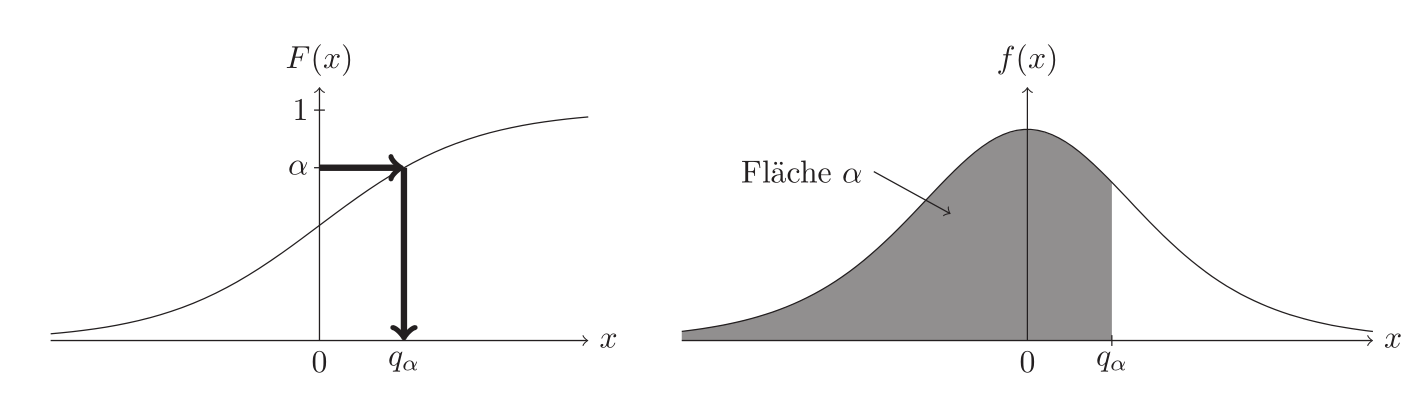
\includegraphics[width=0.8\linewidth]{img/quantile}
\end{center}

\begin{definition}
	The \textbf{sample total} is defined as 
	\begin{equation*}
		S_n = (X_1 + X_2 + \dots + X_n) \sim \mathcal{N}(n\mu, n\sigma_X^2)
	\end{equation*}
	\textbf{Sample mean} is defined by
	\begin{equation*}
		\sample{X}_n = \frac{S_n}{n} \sim(\mu, \frac{\sigma_X^2}{n})
	\end{equation*}
	\textbf{Law of Large Numbers} states that
	\begin{equation*}
		\sample{X}_n \longrightarrow \mu(n\rightarrow \infty)
	\end{equation*}
\end{definition}

% TODO Uniform Distribution

% TODO Exponential Distribution

% TODO Normal Distribution

% TODO Law Of Large Numbers

% TODO Central Limit Theorem

\section{QQ-Plots, Parameter Estimation and t-Tests}

\subsection{QQ-Plot}

A QQ-plot is the empirical quantiles calculated from the data plotted against the theoretical quantiles. If the data is normal distributed the resulting plot has a linear relationship.

\subsubsection{Normal Plot}
\begin{enumerate}[label=(\arabic*)]
	\item Data set $x_1,x_2,\dots, x_n$
	\item $\alpha_k = \frac{k-0.5}{n}\quad k=1,2,\dots,n$
	\item Theoretical Quantile $q(\alpha_k) = \Phi^{-1}(\alpha_k)$
	\item Empirical Quantile $x_{(1)}, x_{(2)},\dots, x_{(n)}$
	\item Plot $\left( q(\alpha_k), x_{(k)} \right)$
\end{enumerate}


\subsection{Parameter Estimation}
\begin{minipage}{0.6\linewidth}
	Once we have verified that a data set follows a presumed distribution, how to estimate the \textbf{parameters} of the distribution from the $n$ observations
	\begin{equation*}
		X_1 = x_1, X_2 = x_2, \dots , X_n = x_n
	\end{equation*}
	For a discrete probability distribution the probability that these $n$ observations or events actually have occurred can be expressed as
	\begin{equation*}
		P[X_1 = x_1] \cdot P[X_2 = x_2] \cdot \dots \cdot P[X_n = x_n] \equiv \prod_{i=1}^{n} P[X_i = x_i]
	\end{equation*}
	The probability that the $n$ independent random variables $x_1,x_2,\dots,x_n$ are observed, depends on the \textbf{parameter $\theta$} which needs to be \textbf{estimated}.
	The Likelihood function $\mathcal{L}(\theta)$ is therefore given by
	\begin{equation*}
		\mathcal{L}(\theta) = \prod_{i=1}^{n} P[X_i = x_i | \theta ]
	\end{equation*}
	where $P[X_i = x_i | \theta ]$ denotes the probability mass function that value $x_i$ has been observed given $\theta$.
\end{minipage}
\begin{minipage}{0.4\linewidth}
	\centering
	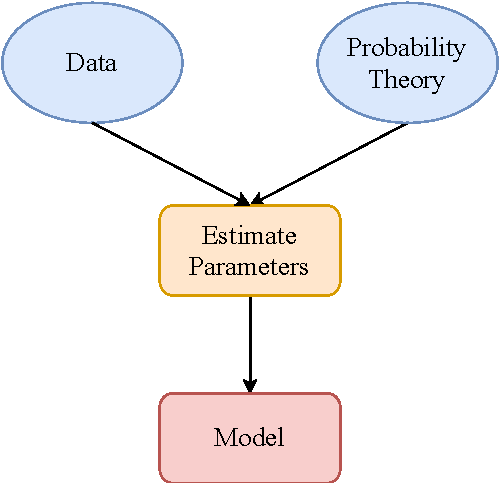
\includegraphics[keepaspectratio, width=0.8\linewidth]{probtheory_model}
\end{minipage}

The idea of \textbf{Maximum Likelihood} is to estimate the parameter $\theta$ in such a way that the \textbf{likelihood is maximised}, that is \emph{makes the observed data most likely or most probable}.

\subsection{Maximum Likelihood Continuous Distribution}
Given a continuous probability distribution  with probability density function $f (x;\theta)$, then the probability that each observation $x_i$ falls into its corresponding interval $[x_i, x_i + \text{d}x_i]$ is
\begin{equation*}
	\prod_{i=1}^{n} f(x_i; \theta) \text{d}x_i
\end{equation*}

Infinitesimal intervals $\text{d}x_i$ do not depend on parameter value $\theta$, they can thus be omitted in the \textbf{likelihood function}

\begin{equation*}
	\mathcal{L} = \prod_{i=1}^{n} f(x_i;\theta)
\end{equation*}

If assumed probability density function $f (x_i ;\theta)$ and parameter value of $\theta$ are correct, we expect a high probability for the actually observed data to occur, which corresponds to a \textbf{maximisation} of $\mathcal{L}(\theta)$.

\subsection{Maximum Likelihood for Exponential Distribution}
Given observation $X_1, X_2, \dots, X_n\text{ i.i.d. }\sim \text{Exp}(\lambda)$, that is $f(x_i;\lambda) = \lambda e^{-\lambda x_i}$. The \textbf{likelihood function} for such a  dataset is given by
\begin{equation*}
	\mathcal{L} = \prod_{i=1}^{n} \lambda e^{-\lambda x_i}
\end{equation*}

The \textbf{Log likelihood} is
\begin{equation*}
	\log(\mathcal{L}(\lambda)) = n\log(\lambda) - \lambda\sum_{i=1}^n x_i
\end{equation*}

\subsection{z-Test}
In the z-Test the value of $\sigma_X$ is known.
\begin{enumerate}
	\item \textbf{Model} $X_i$ is a continuous measurement variable
	\begin{equation*}
		X_i, \dots, X_n \text{i.i.d.} \mathcal{N}(\mu, \sigma_X^2)\quad \sigma_X\text{ known}
	\end{equation*}
	\item \textbf{Null Hypothesis} $H_0: \mu = \mu_0$\\ \textbf{Alternative Hypothesis} $H_A: \mu \neq \mu_0 \text{ or } \mu < \mu_0 \text{ or } \mu > \mu_0$
	\item \textbf{Test statistic}
	\begin{equation*}
		Z = \frac{\sample{X}_n - \mu_0}{\sigma_{\sample{X}_n}} = \frac{\sample{X}_n - \mu_0}{\sigma_X / \sqrt{n}} = \frac{\text{observed} - \text{expected}}{\text{standard error}}
	\end{equation*}
	\textbf{Null distribution} $Z \sim \mathcal{N}(0,1)$
	\item \textbf{Significance Level} $\alpha$
	\item \textbf{Rejection region for test statistic}
	\begin{alignat*}{2}
		K &= (-\infty,z_{\frac{\alpha}{2}}] \cup [z_{1-\frac{\alpha}{2}}, \infty) &\quad \text{ for } H_A : \mu\neq \mu_0\\
		K &= (-\infty, z_\alpha] &\quad \text{ for } H_A : \mu < \mu_0\\
		K &= [ z_{1-\alpha}, \infty ) &\quad \text{ for } H_A : \mu > \mu_0
	\end{alignat*}
	\item \textbf{Test Statistic} Check whether the observed value of the test statistic fall into the rejection region
\end{enumerate}

\begin{definition}
	The \textbf{$p$-value} is the probability that the test statistic will take on a value that is at least as extreme (with respect to the alternative hypothesis) as the observed value of the statistic when the null hypothesis $H_0$ is true.
\end{definition}

\begin{definition}
	\textbf{$p$-value and Test Statistic}: By means of the $p$-value the test decision can be concluded directly: If the $p$-value is smaller than the significance level, then  the null hypothesis $H_0$ is rejected, otherwise it is retained. For a given significance level $\alpha$ a conclusion is drawn on the basis of the $p$-value:
	\begin{enumerate}
		\item Reject $H_0$ if $p$-value $\leq \alpha$
		\item Reject $H_0$ if $p$-value $> \alpha$
	\end{enumerate}
\end{definition}

\subsection{Example: Statistical Test for Average Body Height}
% TODO Example Average Woman's Height



\subsection{Confidence Intervals}
% TODO Confidence Interval



\end{document}
